\documentclass{zc-ust-hw}

\usepackage[]{lipsum} 

\name{SalahDin Ahmed Salh Rezk}
\id{202201079}
\course{Thermodynamics, Wave Motion and Optics}
\assignment{Assignment 4}

\usepackage{import}
\usepackage{xifthen}
\usepackage{pdfpages}

\newcommand{\incfig}[1]{%
    \def\svgwidth{\columnwidth}
    \import{./figures/}{#1.pdf_tex}
}

\newcommand{\midlabelline}[3]{
   \node (midlabel) at ($ (#1)!.5!(#2) $) {#3};
   \draw[<-] (#1) --  (midlabel);
   \draw[->] (midlabel) -- (#2);
}
%% Point
\newcommand{\point}[3]{
\draw[fill=black] (#1) circle (1pt) node[#3] {#2};
}

\usepackage{tikz}

\tikzset{>=latex}
\usetikzlibrary{decorations.markings, calc}

\begin{document}

\maketitle

\begin{enumerate}
  \item For a compound lens system of two thin lenses,
    \begin{enumerate}
      \item Show that the image distance, $S_i$ takes the following form:
        \[
          S_i=\frac{f_{2}d-[f_{1}f_{2}S_{0}/(S_{0}-f_{1})]}{d-f_{2}-[f_{1}S_{0} /(S_{0}-f_{1})]}
        ,\] 
        where $S_0$, $f_1$ and $f_2$ are the object distance and the focal lengths of the system
    \end{enumerate}

    \begin{sol}
      \begin{align}
        \frac{1}{S_{1}} + \frac{1}{S_{0}} &= \frac{1}{f_{1}} 
        \implies
        S_{1} = \frac{S_{0}f_{1}}{S_{0}-f_{1}} \\
        \frac{1}{S_{2}} + \frac{1}{S_{3}} &= \frac{1}{f_{2}} \\
        \intertext{From figure \( S_{2}=d-S_{1} \) and \( S_{3}=S_i \):}
        \frac{1}{d-S_{1}} + \frac{1}{S_i} &= \frac{1}{f_{2}}
        \implies
        S_{i} = \frac{(d-S_{1})f_{2}}{(d-S_{1})-f_{2}} \\
      \end{align}
      \begin{align}
        S_{i} &= \dfrac{(d-\dfrac{S_{0}f_{1}}{S_{0}-f_{1}})f_{2}}{(d-\dfrac{S_{0}f_{1}}{S_{0}-f_{1}})-f_{2}} \\
              &= \dfrac{f_{2}d-\dfrac{f_{1}f_{2}S_{0}}{S_{0}-f_{1}}}{d-f_{2}-\dfrac{S_{0}f_{1}}{S_{0}-f_{1}}}
      .\end{align}
    \end{sol}
  \item Show that the total magnification of the system takes the explicit
    form: 
    \[
      M_T=\frac{f_{2}S_i}{d(S_{0}-f_{1})-S_{0}f_{1}}
    ,\] 
    \begin{sol}
      \begin{align}
        M_{1} &= -\frac{S_{1}}{S_{0}} \\
        M_{2} &= -\frac{S_{3}}{S_{2}} \\
        M_T &= M_{1} M_{2} \\
            &= \frac{S_{1}S_{3}}{S_{0}S_{2}}
      .\end{align}
      \newpage
      Using \( S_{2}=d-S_{1} \), \( S_{3}=S_i \), and formulas from previous part:
      \begin{align}
        M_T &= \frac{S_{1}S_{i}}{S_{0}(d-S_{1})} \\
            &= \frac{\frac{S_{0}f_{1}}{S_{0}-f_{1}}S_{i}}{S_{0}(d-\frac{S_{0}f_{1}}{S_{0}-f_{1}})} \\
            &= \frac{S_{0}f_{1}S_{i}}{(S_{0}-f_{1})S_{0}(d-\frac{S_{0}f_{1}}{S_{0}-f_{1}})} \\
            &= \frac{S_{0}f_{1}S_{i}}{(S_{0}-f_{1})(S_{0}d-S_{0}\frac{S_{0}f_{1}}{S_{0}-f_{1}})} \\
            &= \frac{S_{0}f_{1}S_{i}}{(S_{0}-f_{1})S_{0}d-S_{0}S_{0}f_{1}} \\
            &= \frac{f_{1}S_{i}}{(S_{0}-f_{1})d-S_{0}f_{1}}
      .\end{align}
    \end{sol}

    \newpage

  \item Show that for a thin lens immersed in a medium of refractive index nm,
    the Lensmaker equation takes the following form.
    \[
      \frac{1}{f} = \frac{n_{l}-n_{m}}{n_{m}} \left( \frac{1}{R_{1}}-\frac{1}{R_{2}} \right) 
    .\] 
    where \( n_{l} \) is the index of refraction of glass.
    
    \begin{figure}[H]
      \begin{center}
        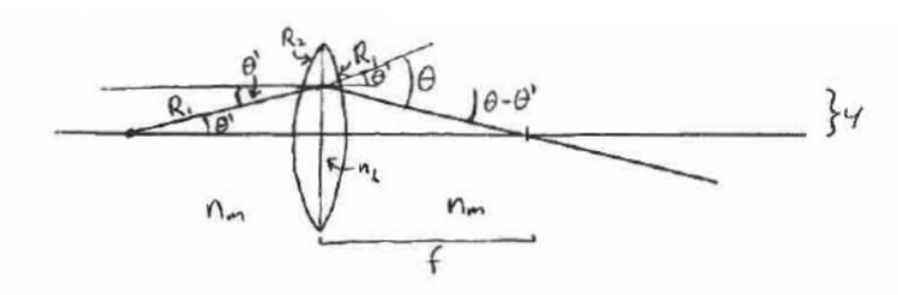
\includegraphics[width=0.95\textwidth]{figures/1705960477.png}
      \end{center}
      \caption{}
    \end{figure}
    
    \begin{sol}
      For \( \theta \ll 1 \)
      \begin{gather}
        \frac{y}{R_{1}} = \sin \theta' \approx \theta' \\
        n_l\sin \theta' = n_m\sin \theta \implies n_l\theta'=n_m\theta \\
        \theta -\theta' = \left( \frac{n_l}{n_m}-1 \right) \theta' = \left( \frac{n_l}{n_m}-1 \right) \frac{y}{R_{1}} \\
        f=\frac{y}{\tan (\theta -\theta')} \approx \frac{y}{\theta -\theta'} = \frac{R_{1}}{\frac{n_l}{n_m}-1} = \frac{n_mR_{1}}{n_l-n_m} \\
        \frac{1}{f} = \frac{n_l-n_m}{n_m} \frac{1}{R_{1}}
        \intertext{The other lens will add linearly}
        \frac{1}{f} = \frac{n_l-n_m}{n_m} \left( \frac{1}{R_{1}} + \frac{1}{R_{2}} \right) 
      .\end{gather}
    \end{sol}
    
    \newpage
    
  \item The passenger side rear view mirror of a car has a sign ``Objects in the
    mirror are closer than they appear''. Can we conclude if the mirror is
    convex or concave? If an object located 100 m away appears 125 m away, what
    is the radius of the mirror?
    \begin{sol}
      Concave, since it forms a virtual large image for objects between focus
      and mirror, so for mirrors with large focal lengths it will preform the
      desired effect.
      \begin{align}
        \frac{1}{f} &= \frac{1}{s} + \frac{1}{s'} \\
        f &= \frac{ss'}{s+s'} \\
        &= \frac{-100*125}{100-125} \\
        &= 500
      .\end{align}
    \end{sol}

  \item Imagine a stratified system consisting of $m$ planar layers of
    transparent materials of different thickness. Show that the propagation
    direction of the emerging beam is determined by only the incident direction
    and the refractive indices of the initial and final layers, i.e., $n_1$ and $n_m$
    \begin{sol}
      \begin{align}
        n_{1}\sin \theta_{i 1} &= n_{2}\sin \theta_{t 2} \\
        n_{1}\sin \theta_{i 2} &= n_{2}\sin \theta_{t 3} \\
        &\vdots \\
        n_{\ell}\sin \theta_{i \ell} &= n_{m}\sin \theta_{m} \\
        \intertext{Notice \( \theta_{t 2}=\theta_{i 2},\theta_{t 3}=\theta_{i 3} \)}
        n_{1}\sin \theta_{i 1} = n_{2}\sin \theta_{i 2} = &\ldots = n_{\ell}\sin \theta_{i \ell} = n_{m}\sin \theta_{m}
      .\end{align}
      Therefore \( n_{1}\sin \theta_{i 1} = n_m\sin \theta_{tm} \)
    \end{sol}

    \newpage

  \item A small fish, four feet below the surface of Lake Mendota is viewed
    through a simple thin converging lens with focal length 30 feet. H the lens
    is 2 feet above the water surface (as shown in Fig.), where is the image of
    the fish seen by the observer? Assume the fish lies on the optical axis of
    the lens and that $n_\text{air}$ = 1.00, \(n_\text{water}\) = 1.33. 
    \begin{figure}[H]
      \begin{center}
        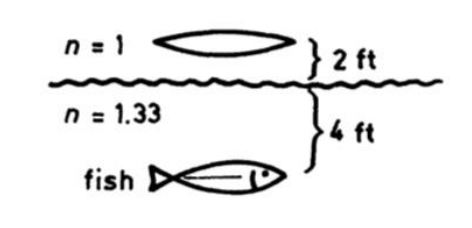
\includegraphics[width=0.35\textwidth]{figures/1705961934.png}
      \end{center}
      \caption{}
    \end{figure}

    \begin{sol}
      \begin{align}
        1.33\sin \theta_{1} &= \sin \theta_{2} \\
        \intertext{For \(\theta \ll 1\)}
        1.33\theta_{1} &= \theta_{2} \\
        1.33 \frac{y}{R_{1}} &= \frac{y}{R_{2}} \\
        1.33 \frac{1}{R_{1}} &= \frac{1}{R_{2}} \\
        R_{2} &= \frac{R_{1}}{1.33} \\
              &= 3 \\
        u &= 2 + R_{2} \\
          &= 5 \\
        \frac{1}{f}&=\frac{1}{u}+\frac{1}{v} \\
        v&= -6
      .\end{align}
      The image of the fish will appear as is.
    \end{sol}

    \newpage

  \item It is said that: ``In normal use, the magnitude of the magnification of
    an imaging system increases as its equivalent focal length is increased.''
    Find an expression for the magnification in terms of the focal length that
    demonstrates the truth or falsehood of this statement. State any conditions
    that must be satisfied in the mathematical expression (e.g., why does the
    sentence include the caveat ``in normal use''?). 
    \begin{sol}
      \begin{align}
        M_T&=-\frac{s'}{s} \\
        \frac{1}{f} &= \frac{1}{s}+\frac{1}{s'} \\
        s' &= \frac{sf}{s-f} \\
        M_T &= -\frac{\left( \frac{sf}{s-f} \right) }{s} \\
        &= \frac{f}{f-s} \\
        &= -\frac{f}{s}\left( \frac{1}{1-\frac{f}{s}} \right)  \\
        \intertext{For \( f<s \) we can use $\frac{1}{1-t}=\sum_{n=0}^{\infty} t^n$ where \( t<1 \)}
        M_T &= -\sum_{n=1}^{\infty} \left( \frac{f}{s} \right)^{n} 
        \intertext{For \( f \ll s \)}
        M_T &\approx -\frac{f}{s}-\frac{f^2}{s^2}
      .\end{align}
      Therefore \( M_T \propto f,f^2 \) for \( f \ll s \).
    \end{sol}

    \newpage
  \item As shown in the figure below, a thin converging lens of focal length 14
    cm forms an image of the square $abcd$, which is $hc = hb = 10$ cm high and
    lies between distances of $pd = 20$ cm and $pa = 30$ cm from the lens. \\
    Let $a', b', c',$ and $d'$ represent the respective corners of the image.  
    Let $qa$ represent the image distance for points $a'$ and $b'$, $qd$ represent 
    the image distance for points $c'$ and $d'$, $h'b$ represents the distance 
    from point $b'$ to the axis, and $h'c$ represent the height of $c'$.
    \begin{enumerate}
      \item Evaluate each of the quantities written in bold.
        \begin{sol}
          \begin{align}
            \frac{1}{p_a}+\frac{1}{q_a}&=\frac{1}{f} \\
            \frac{1}{30}+\frac{1}{q_{1}}&=\frac{1}{14} \\
            q_{1} &= 26.2 \\
            h_b'&=hM_a=h \left( -\frac{q_a}{p_a} \right) \\
            &= (10.0\text{ cm})(-0.875)=-8.75\text{ cm} \\
            \frac{1}{20}+\frac{1}{q_d}&=\frac{1}{14}
            q_d &= 46.7\text{ cm}
          \end{align}
        \end{sol}
      \item Make a sketch of the image.
        \begin{sol}\end{sol}
        \begin{figure}[H]
          \begin{center}
            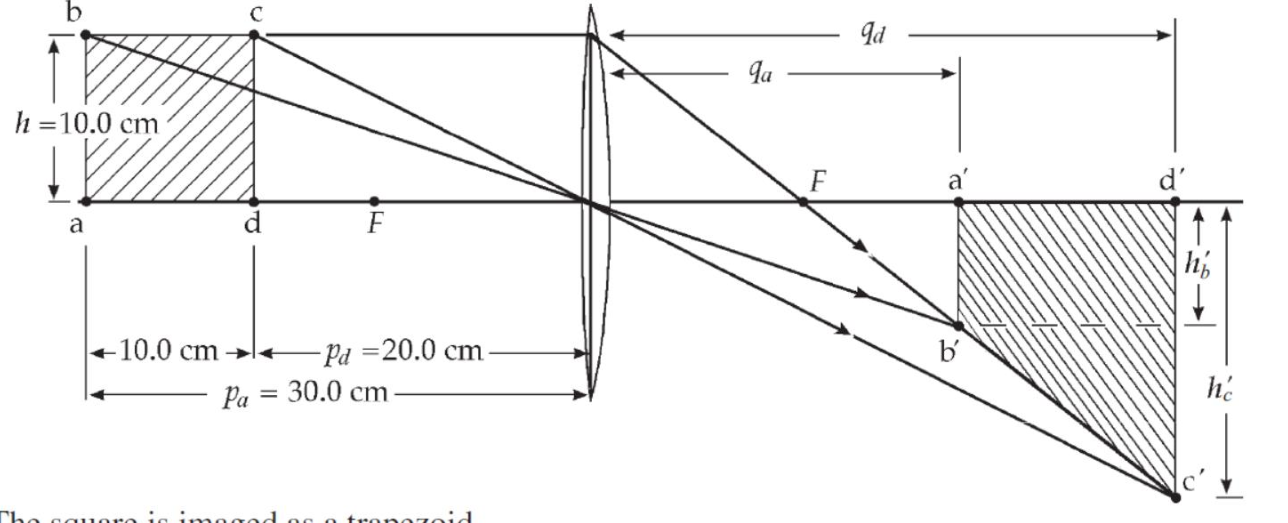
\includegraphics[width=0.95\textwidth]{figures/1705970086.png}
          \end{center}
          \caption{}
        \end{figure}
        
      \item Calculate the area of the image using the results of (a) and (b).
        \begin{sol}
          \begin{align}
            \frac{(h_c'+h_b')(qd-qa)}{2}= 238\text{ cm}^2
          .\end{align}
        \end{sol}
      \item Let $q$ represent the image distance of any point between $a'$ and $d'$,
        for which the object distance is $p$. Let $h'$ represent the distance from
        the axis to the point at the edge of the image between $b'$ and $c'$ at
        image distance $q$. Show that 
        \[
          |h'|=(10\text{ cm})q\left(\frac{1}{14\text{ cm}}-\frac{1}{q}\right) 
        .\] 
        \begin{sol}
          \begin{align}
            \frac{1}{p}+\frac{1}{q}&=\frac{1}{f} \\
            \frac{1}{p}+\frac{1}{q}&=\frac{1}{14} \\
            |h'| = |hM| &= |h \left( -\frac{q}{p} \right) \\
                        &= (10.0\text{ cm})q \left( \frac{1}{14\text{ cm}}-\frac{1}{q} \right) 
          .\end{align}
        \end{sol}
      \item Explain why the geometric area of the image can be given by
        \[
          \int_{q_a}^{q_d} |h^*|dq 
        .\] 
        \begin{sol}
          Because integration gives the area under the region.
        \end{sol}
      \item Calculate the area of the image using integration above.
        \begin{sol}
          \begin{align}
& \int_{q_a}^{q_d}\left|h^{\prime}\right| d q=\int_{q_a}^{q_d}(10.0
            \mathrm{~cm})\left(\frac{q}{14 \mathrm{~cm}}-1\right) d q=(10.0
            \mathrm{~cm})\left(\frac{q^2}{28 \mathrm{~cm}}-q\right)_{26.2
          \mathrm{~cm}}^{46.7 \mathrm{~cm}} \\ & \text { Area }=(10.0
          \mathrm{~cm})\left(\frac{46.7^2-26.2^2}{28}-46.7+26.2\right)
          \mathrm{cm}=328 \mathrm{~cm}^2
          .\end{align}
        \end{sol}
    \end{enumerate}
    
    \newpage
    
  \item A thin equi-convex lens of glass of refractive index ng= 3/2 and of
    focal length 0.3 m in air is sealed into an opening at one end of a tank
    filled with water nw = 4/3. On the opposite side of the lens, a mirror is
    placed inside the tank on the tank wall perpendicular to the lens as shown
    in the figure below. The separation between the lens and the mirror is 0.8
    m. A small object is placed at a distance of 0.9 m from the lens as shown
    in the figure.  

    Find the position (relative to the lens) of the image of the object formed
    by the system.  
    \begin{figure}[htpb]
      \begin{center}
        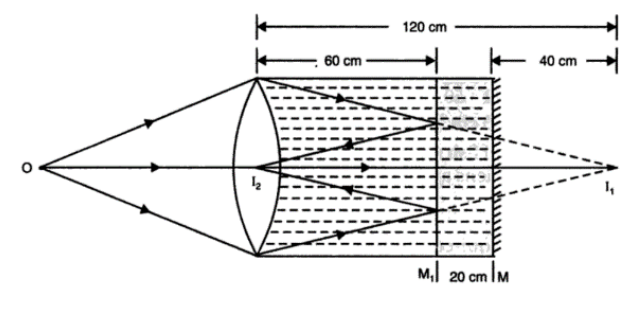
\includegraphics[width=0.5\textwidth]{figures/1705970589.png}
      \end{center}
      \caption{}
    \end{figure}

    \begin{sol}
      \begin{align}
        \frac{n 1}{s}+\frac{n 2}{s^{\prime}}&=\frac{n 2-n 1}{R} \\
        \frac{3 / 2}{s^{\prime}}+\frac{1}{0.9}&=\frac{0.5}{0.3} \\
        s^{\prime}&=2.7 \mathrm{~m} \\
        \frac{\frac{4}{3}}{s^{\prime \prime}}-\frac{\frac{3}{2}}{2.7}&=\frac{\frac{4}{3}-\frac{3}{2}}{-0.3}\\
        \frac{4}{3 s^{\prime \prime}}&=\frac{1}{1.8}+\frac{1}{1.8}=\frac{1}{0.9} \\
        s^{\prime \prime}&=1.2 \mathrm{~m} \\
        x&=\left(1-\frac{1}{n_{\text {water }}}\right) \\
        x_0&=\left(1-\frac{3}{4}\right) 0.8 . \\
           &=0.2 \mathrm{~m}
      .\end{align}
    \end{sol}
    
\end{enumerate}

\end{document}
